\documentclass{article}

\usepackage{graphicx}
\usepackage{tikz}
\usepackage{tikzsymbols}
\usetikzlibrary{calc,patterns,shapes.geometric}
\pagestyle{empty}
\usepackage[margin=0pt]{geometry}
\geometry{papersize={14in,12in}}

\def\centerarc[#1](#2)(#3:#4:#5){\draw[#1] ($(#2)+({#5*cos(#3)},{#5*sin(#3)})$) arc (#3:#4:#5);}

\begin{document}
	\begin{figure}
		\centering
		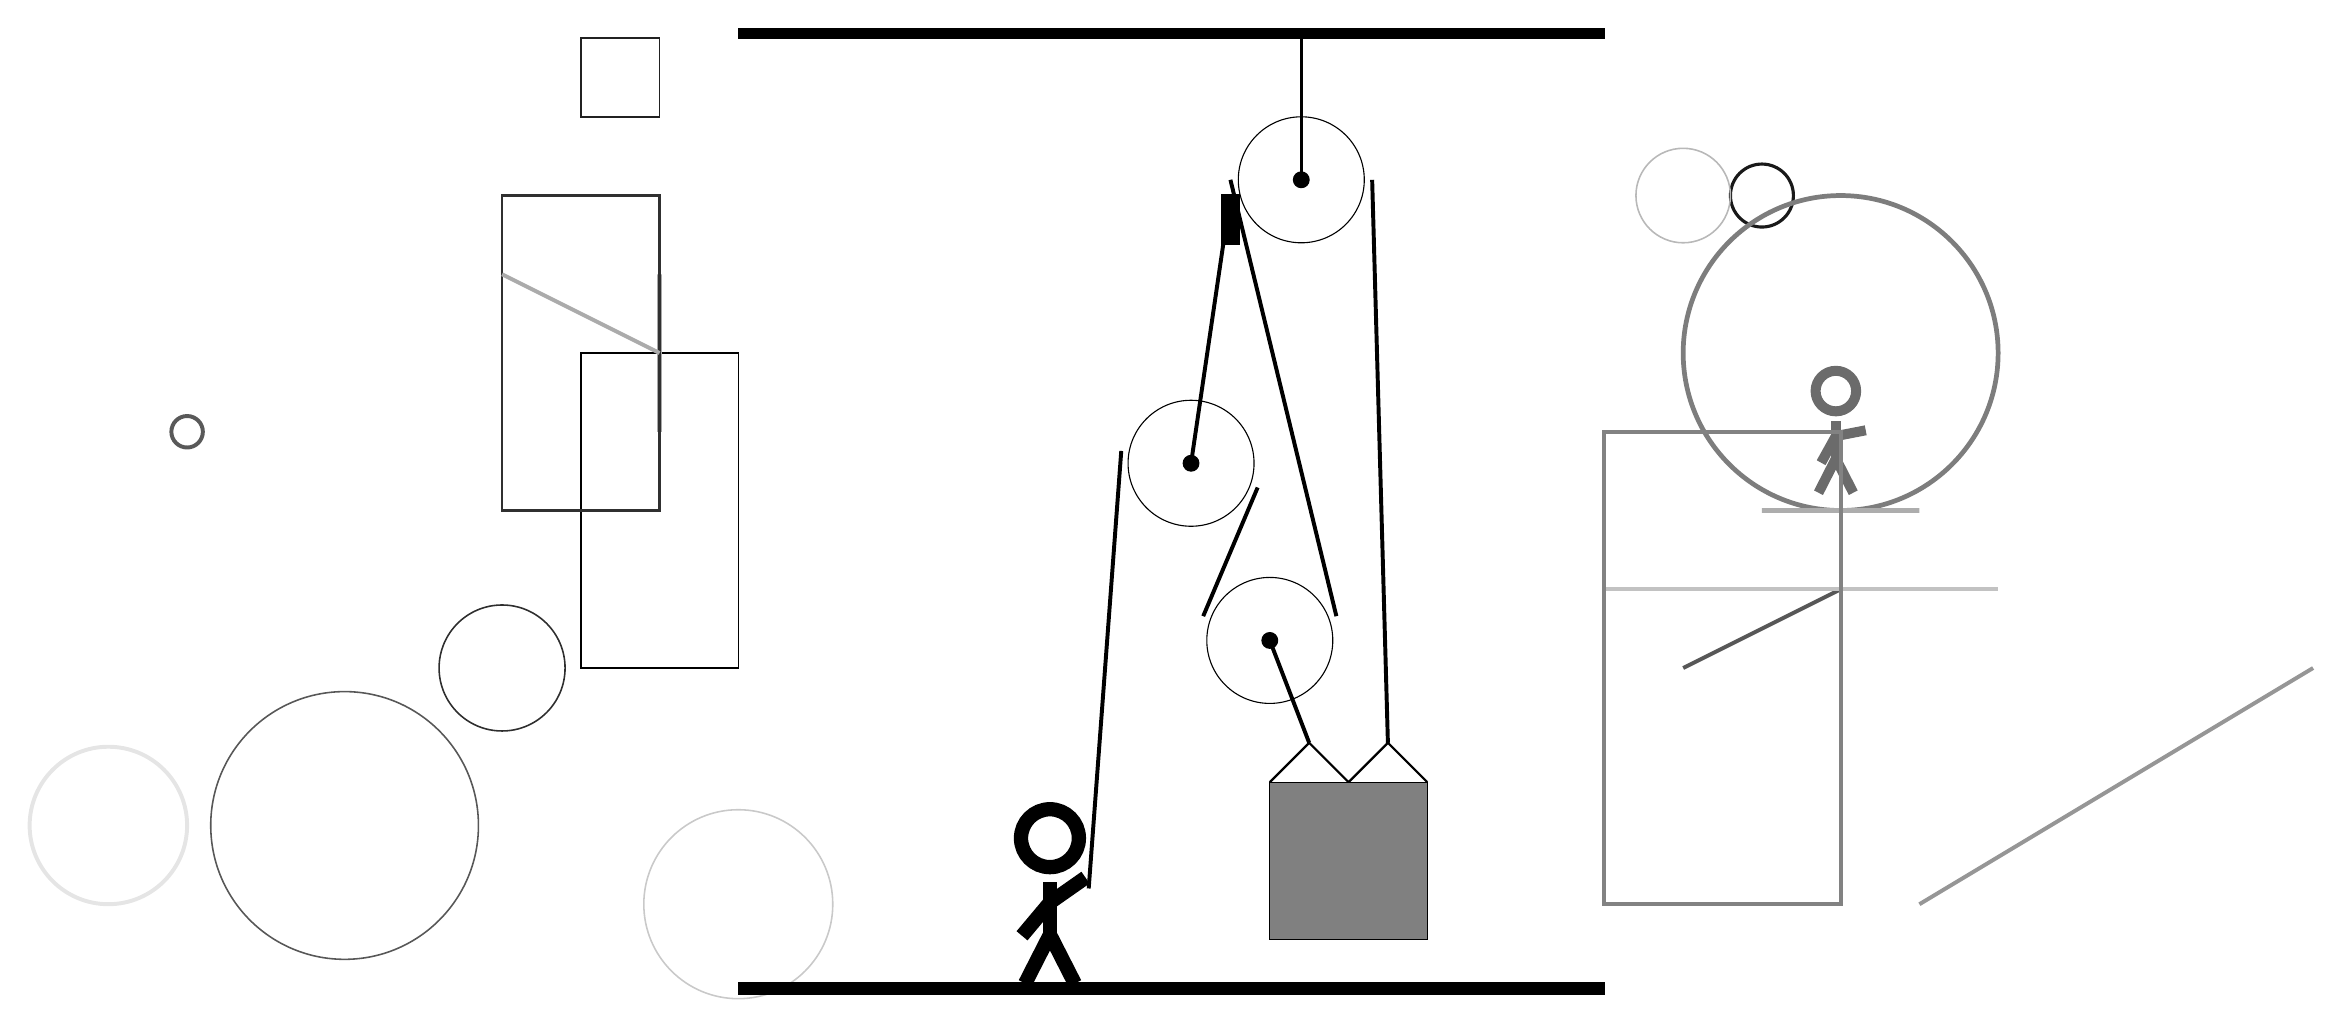
\begin{tikzpicture}
			%%%%% START %%%%%
			
			\draw[fill=black] (-6, 9) rectangle (5, 9.125);
			
			\draw (-0.25, 3.6) circle (0.8);
			\draw[fill=black] (-0.25, 3.6) circle (0.1);
			
			\draw[line width=0.5mm, color=black!41](9, -2) -- (14, 1);
			
			\draw [line width=0.4mm, color=black!90](7, 7) circle (0.4);
			\draw [line width=0.5mm, color=black!10](-14, -1) circle (1.0);
			\draw[line width=0.2mm, color=black!100] (-8, 5) rectangle (-6, 1);
			\draw [line width=0.6mm, color=black!51](8, 5) circle (2.0);
			
			\node[line width=0.4mm, color=black!58] at (8, 4) {\Strichmaxerl[7][61][11]};
			
			\draw[line width=0.6mm, color=black!32] (7, 3) rectangle (9, 3);
			
			\draw[line width=0.2mm, color=black!87] (-8, 9) rectangle (-7, 8);
			\draw[line width=0.5mm, color=black!66](6, 1) -- (8, 2);
			\draw[line width=0.5mm, color=black!24](5, 2) -- (10, 2);
			
			\draw[line width=0.7mm, color=black!34] (-7, 6) rectangle (-7, 4);
			
			\draw[line width=0.3mm, color=black!81] (-7, 3) rectangle (-9, 7);
			\draw [line width=0.2mm, color=black!21](-6, -2) circle (1.2);
			
			\draw [line width=0.2mm, color=black!28](6, 7) circle (0.6);
			\draw [line width=0.2mm, color=black!82](-9, 1) circle (0.8);
			\draw [line width=0.7mm, color=black!18](6, -3) circle (0.0);
			\draw[line width=0.5mm, color=black!49] (5, -2) rectangle (8, 4);
			\draw[line width=0.6mm, color=black!41] (7, 4) rectangle (7, 4);
			\draw [line width=0.5mm, color=black!65](-13, 4) circle (0.2);
			\draw [line width=0.2mm, color=black!66](-11, -1) circle (1.7);
			\draw[line width=0.5mm, color=black!33](-9, 6) -- (-7, 5);
			
			
			\draw (0.75, 1.35) circle (0.8);
			\draw[fill=black] (0.75, 1.35) circle (0.1);
			
			\draw (1.15, 7.2) circle (0.8);
			\draw[fill=black] (1.15, 7.2) circle (0.1);
			\draw[very thick] (1.15, 7.2) -- (1.15, 9);
			
			\draw[thick]  (0.75, -0.45) -- (1.25, 0.05) -- (1.75, -0.45) -- (2.25, 0.05) -- (2.75, -0.45);
			\draw[fill=black!50] (0.75, -0.45) rectangle (2.75, -2.45);
			
			\draw[line width=0.5mm] (-0.25, 3.6) -- (0.25, 7.0);
			\draw[line width=0.5mm, fill=black](0.15, 6.4) rectangle (0.35, 7.0);
			\draw[line width=0.5mm] (-1.55, -1.8) -- (-1.1363, 3.7562);
			\centerarc[line width=0.5mm](-0.25, 3.6)(-20:170:0.9);
			\draw[line width=0.5mm] (0.5957, 3.2922) -- (-0.0957, 1.6578);
			\centerarc[line width=0.5mm](0.75, 1.35)(160:380:0.9);
			\draw[line width=0.5mm] (1.5957, 1.6578) -- (0.25, 7.2);
			\draw[line width=0.5mm](0.75, 1.35) -- (1.25, 0.05);
			\centerarc[line width=0.5mm](1.15, 7.2)(0:180:0.9);
			\draw[line width=0.5mm] (2.05, 7.2) -- (2.25, 0.05);
			
			\node at (-2, -1.9) {\Strichmaxerl[10][50][35]};
			
			\draw[fill=black] (-6, -3) rectangle (5, -3.15);
			
			%%%%% END %%%%%
		\end{tikzpicture}
	\end{figure}	
\end{document}